\documentclass[conference]{IEEEtran}
\IEEEoverridecommandlockouts
\usepackage{cite}
\usepackage{amsmath,amssymb,amsfonts}
\usepackage{algorithmic}
\usepackage{dsfont}
\usepackage{graphicx}
\usepackage{textcomp}
\usepackage{xcolor}
\def\BibTeX{{\rm B\kern-.05em{\sc i\kern-.025em b}\kern-.08em
    T\kern-.1667em\lower.7ex\hbox{E}\kern-.125emX}}
\begin{document}

\title{Video Object Segmentation - Implementation of YouTube VOS\\
}

\author{\IEEEauthorblockN{1\textsuperscript{st} Sudipta Mandal}
\IEEEauthorblockA{\textit{1721489042} \\
}
\and
\IEEEauthorblockN{2\textsuperscript{nd} Shad Al Kaiser}
\IEEEauthorblockA{\textit{1721392042}\\
}
\and
\IEEEauthorblockN{3\textsuperscript{rd} Ashraful Kalam Abid}
\IEEEauthorblockA{\textit{1721464042} \\
}
}

\maketitle

\begin{abstract}
The dataset of YouTube-VOS is dominating the field of Video Object Segmentation. Though there are many research paper or proposed method on video object segmentation but the implementations of those paper are rare. There are some GitHub repos based on Video Object Segmentation but they require powerful machine to run the project. In this project we tried to re-implement a repository like that. The repo didn’t run well in google-colab. We had to re-adjust the training model’s tensor dimension of the RGB images to make the model compatible with the test data. We proposed a simple routing file to easily make all the paths to the root. Made the project easily compatible to run in google-colab. We have run the full train dataset as well as the full test dataset of YouTube-VOS. Finally, experiments showed that our implemented model is fully running as we got a score from the google coda lab challenge on YouTube-VOS.
\end{abstract}

\begin{IEEEkeywords}
Video Object Segmentations, sequence-to-sequence, Large-scale Dataset, Spatial-Temporal, Routing File, Tensor Dimension, YouTube-VOS, Google-Colab, GitHub, Repo.
\end{IEEEkeywords}

\section{Introduction}
Video in general is very popular medium of media right now. To understand a video, video object segmentation plays an important role. Therefore, learning effective analysis to understand video we have chosen to do our work on video object segmentation. For analyzing a video analysis task, learning effective spatial-temporal features is considered to be very important. For our research we took a look into the paper YouTube-VOS where the authors proposed a sequence-to-sequence video object segmentation\cite{xu2018youtube}.\newline
In the YouTube-VOS paper they mentioned about many methods to do objectify videos. Donahue el al.\cite{donahue2015long} proposed unsupervised LSTM autoencoder is one of them. In their work they developed a 3D convolutional network. This convolutional network jointly extracts spatial and temporal information from a video. Video Object Segmentation mainly targets a particular object medium from a video. By going frame to frame it mask different object in different masks.\newline
Based on the YouTube-VOS paper we followed; they proposed a new way to develop a learning algorithm. It will explore sequence-to-sequence spatial-temporal modeling for video object segmentation. By encoding image frame from convolutional LSTM\cite{shi2015convolutional}, it outputs an encoded spatial-temporal information of an image frame in more of an end-to-end manner. The model outputs a segmentation mask of the image. The main idea of the research was very interesting so we decided to implement their work based on the paper.
To implement the work, we choose a GitHub repository\cite{Vkt} to begin with. This repository was the implementation of the paper we talked about earlier. The repo was based on a local machine. Our goal was to make the project compatible with Google-Colab. We made a subset of the main training dataset and successfully trained the model with the training subset.
But when to test the model we had found an issue with the repository. The implantation was faulty as the tensor dimension of the train model and test data were different. It couldn’t able to test the model with the test data because of the incapability of image dimension. Then we came up with a simple solution to solve the issue. By routing all the path to the root first we made it easier to navigate in google-colab. Then we masked the last two RGB dimension of the trained model into a single one. Our approach solved the issue with testing the model and it 

\vspace{.5cm}
\section{Literature Review}
\subsection{Fast End-to-End Embedding Learning for Video Object Segmentation.} 
The approach taken for this method is FEELVOS.\cite{voigtlaender2019feelvos} It's goal is to make the VOS process a bit more simple. To achieve simplicity they had to sacrifice fine tuning. The reasoning for ditching fine tuning was, even though many successful models rely on fine tuning using first frame of the annotation or ground truth, the tuning usually has a high run time and not suitable for most practical applications.\\
The author set out to get a semi supervised VOS method with 4 fundamentals, simple, fast, strong and end-to-end. the implementation of this model was done on the DAVIS\cite{binas2017ddd17} datasets. The goal of this design was to get a better efficiency without using fine tuning and the results can back that up. This model ticked more boxes than PReMVOS\cite{luiten2018premvos} and ONaVOS\cite{voigtlaender2017online}, both of these methods use fine tuning.\\
The FEELVOS method learns pixel-wise embedding using the PML\cite{chen2018blazingly}(Pixel-wise Metric Learning). Using PML, the model becomes much faster and simpler than before. The model also make use of the "Nearest Neighbor" matching as internal guidance of convolutional network instead of using is for final segmentation decision. The network can recover from slightly incorrect answer because it only uses nearest neighbor mechanism as a soft cue.\\
The FEELVOS\cite{voigtlaender2019feelvos} model was brought on to make the designing easy and increase the practical usability. Despite not using fine tuning it was able to show a strong performance on DAVIS 2017 datasets. The structure of the design make it effective, efficient and not time consuming as compared to some of the other existing models.
\subsection{Video Object Segmentation with First-Frame Fine-tuning.} There are many approaches for semi supervised VOS that are based on fine tuning of the first frame. OSVOS\cite{caelles2017one} rely on fine tuning the first frame ground truth using a convolutional network. OnAVOS\cite{voigtlaender2017online} and OSVOS-S\cite{maninis2018video} also follow this method but they also extend it to online adaptation. Learning to propagate through segment masks using optical flow can be another way of implementing this. MaskTask\cite{koike2020learning} and LucidTracker\cite{khoreva2017lucid} extended this idea and introduced an elaborated data augmentation mechanism. MaskedRNN\cite{hu2017maskrnn}, a method that follows recurrent neural network to fuse and redefine the output of two deep networks. 
\subsection{Video Object Segmentation with First-Frame Fine-tuning.} There are many approaches for semi supervised VOS that are based on fine tuning of the first frame. OSVOS\cite{caelles2017one} rely on fine tuning the first frame ground truth using a convolutional network. OnAVOS\cite{voigtlaender2017online} and OSVOS-S\cite{maninis2018video} also follow this method but they also extend it to online adaptation. Learning to propagate through segment masks using optical flow can be another way of implementing this. MaskTask\cite{koike2020learning} and LucidTracker\cite{khoreva2017lucid} extended this idea and introduced an elaborated data augmentation mechanism. MaskedRNN\cite{hu2017maskrnn}, a method that follows recurrent neural network to fuse and redefine the output of two deep networks. 
\subsection{Visual Object Tracking.}
The popular approach for VOS until recent years was to train the model from ground truth of the first frame of the video. The training of an online discriminative classifier and the updating it online is known as tracking by detection. A simple algorithm known as "Correlation Filter" allows to discriminate between template of the target and its 2D translations. This strategy was popularized and risen to prominence by notable effort from Bolme \emph{et al.} \cite{bolme2010visual}. The performance of this method has been improved later by the use of multi channel  formulation, spatial constrains and deep features. There is also a different approach to video tracking objects. This approach utilizes the offline training on similarity functions on pairs of videos\cite{bertinetto2016fully}. There is noticeable improvement on tracking performance by making use of region proposals, hard negative mining, ensembling and memory networks. Most of the tracking methods use rectangle bounding box to initiate the target and to calculate it's position in the subsequent frames. It does not represent the target object sometimes as intended.
\subsection{FCNs for Segmentation.} There has been an immense advancement in image recognition in recent years and it has helped the segmentation process quite a bit. Fully Convolutional Networks(FCN)\cite{long2015fully} has improved the dense predictions with CNNs. They proposed a change of last layer to 1x1 convolution and found that it was possible to train on images of arbitrary sizes. By doing that it would increase the efficiency while performing redundant computation in overlapping patches. CNN architects are of nature where the activation of intermediate layers decrease in size as spatial pooling operation happens. Making prediction from that result in coarsely localized outputs. Activation from shallow layers are later put in to prediction to localize the outcome. 


\subsection{One Shot Video Object Segmentation.} One Shot Video object segmentation or known as OSVOS\cite{caelles2017one} is formed on the basic of fully convolutional neural networks. The process is semi supervised, when the objects in the videos move away from their background. The model is able to transfer the info it take from ImageNet, to the foreground segmentation then learn the appearance of the objects in the video of a single annotation, that is why it is called One Shot. In OSVOS what the model really does is it makes background and foreground from all the pixels of the video. The successfully execute  this the authors focused on adaptaion of CNN to a single instance where a single manual annotation is given.\\
After that the process of fine tuning begins on specific objects that were previously manually segmented. The model process individual frame so every frame of the video becomes independent. By doing that the by-product achieve temporal consistency. It is possible in OSVOS to process each frames not in sequence because it can segment object by occlusions.\\
OSVOS can tackle the trade-offs among time and speed. The level of fine tuning can be increased or decreased at will, faster results or more accurate outcome, whichever we prefer. If we add more annotations manually it can refine and tune the model even more to predict a better outcome. Their study has shown that with 2 annotation it had 84.6\% result but with 4 annotated frames, it jumped to 86.9\%. The experiments were done on DAVIS and YouTube-Objects\cite{xu2018youtube} data sets.



\subsection{Fast Video Object Segmentation - Reference Guided Mask Propagation.}
Using the mask propagation and object detection, this model builds a Siamese encoder-decoder network. The training itself is two staged and works with both online and offline learning. The lack of bigger segmented data sets is the reason behind the 2 stage of schemes for the data. The scheme pre-trains the image data into video data. In a sense this is a hybrid method because it make use of both previous mask and the reference frame of object to propagate the current frame.
One notable thing here is the post-processing which is not time consuming. Thats why the usual test time efficiency is great on this proposed model. The model did achieve state-of-the-art performance on public benchmarks. 


\subsection{Fast Video Object Segmentation - A Unifying Approach.}
This model described how to object tracking and semi supervised video segmentation in real time. The method SiamMask\cite{wang2019fast} redefine offline training of the previously mentioned Siamese approach for object tracking. The method is based on a single bounding box initialisation. It is quite simple in it's way but versatile and efficient at the same time. The inspiration for this model yields from fast tracking Siamese network's success. It focuses on maintaining the offline training and online feasibility of that methods but improving the fine tuning and their target object representation.\\
Modifying the Siamese mask to train it with three task is the first step of a SiamMask model, each of the task has different strategy and their intent is to co relate between target object and the candidate regions of the new frame. The other tasks are the regression of bounding box with the help of Region Proposal Network and class-agonistic binary segmentation that is only needed for offline training session. \\
After that training period the model is only dependent on single box initialization that rotates at 55fps. To validate it's efficiency, the model establishes a state-of-art in VOT-2018 for real time tracking. One of the advantages of this model is it does not require any online update or any kind of adaptation whatsoever yet still performs brilliantly.



\subsection{Zero-Shot Video Object Segmentation via Attentive Graph Neural Networks
.} ZVOS\cite{wang2019zero} is a model that use a Novel Attentive Graph Neural Network(AGNN). AGNN's main goal is to present the video frames as a fully connected graphs. By doing that the frames can be interpreted as nodes of that graph. Thus the relationship between frames are found using nodes and edges to mine and find the connection between them. More testing and validation with extending AGNN shows that the model itself set a new state-of-the-art. \\
AGNN casts ZVOS as end-to-end message passing based graph. VOS is a per pixel prediction thing and the AGNN technique is suited for that because it is able to preserve spatial information. The model works with multiple layers so that AGNN can contribute to neural training data augmentation. The model was tested on DAVIS\cite{binas2017ddd17}  and YouTube-Objects\cite{xu2018youtube} data sets.\\
The ability of AGNN being differential makes it easy for the users to pass high-order edges, which are the relations between frames in this model because the frames are like nodes. To refine the model image object co-segmentation(ICOS) was tested and it showed that it is possible to distinguish general targeted objects from the group of related images. The authors attempted to utilize GNN to overcome the task which was predicting from pixel-wise segmentation. The importance of this kind of early attempts can be demonstrated by getting a favorable results in state-of-the-art methods, which the model did.  


\subsection{AGSS-VOS: Attention Guided Single-Shot Video Object Segmentation.} With the models we have reviewed so far most of them process the targeted objects separately. AGSS-VOSS\cite{Lin_2019_ICCV} approaches the object segmentation in a different way. To segment multiple objects at once it forwards one feed by using instance-agnostic and instance-specific modules. A attention guided decoder is used to fuse the data from multiple modules.\\
The purpose of the adaptation of instance-agnostic is to gather all the information shared by all the instances. The instance-specific is used to generate the features for those instances. Those two modules give outputs that are then fused by the attention guided decoder. The final information is then used to generate mask for instances and then normalized to make the object segmentation predictions.
The model is time saving when we consider that it compute the references and the frames of all the targets in one instance-agnostic module. But it rarely compromises the accuracy of the predictions. The experiment was on the DAVIS\cite{binas2017ddd17} and YouTube-VOS\cite{xu2018youtube} data sets.



\subsection{UnOVOST: Unsupervised Offline Video Object Segmentation and Tracking.} To tackle the difficulties for generating masks for unsupervised video object segmentation and tracking the objects this model proposed UnVOST\cite{Luiten_2020_WACV} algorithm. The workflow is divided in some stages. Starting with grouping the segments and then merging those to make a consistent long term object track based on the visual similarity. Forest Path Cutting algorithm is used to get a decision tree to form these long term tracklets. The model showed exceptionally well results on DAVIS data sets for unsupervised data sets, placing at the 1st place.
In an unsupervised setting the model needs to get all the objects and the tracks and segments right. UnOVOST is an algorithm that builds up object segmentation tracks while working on multiple stages. The masking of these frames are done using Mask R-CNN\cite{he2017mask}.\\
Two cues are responsible for segment tracking, those are the spatio-temporal consistency of the mask
segments in contiguous frames under optical flow warping,
and the appearance-based visual similarity of the mask segments encoded as an object re-identification vector. These are merged in the second stages of the model to get the long term consistent tracks.
The undeniable efficiency of this UnOVOST model makes it the best model for unsupervised video segmentation. 



\subsection{MoNet: Deep Motion Exploitation for Video Object Segmentation.}
The purpose of using MoNet\cite{Xiao_2018_CVPR} is to enhance two aspects of Video Object Segmentation. Those are frame representation learning and segment refinement. MoNet takes advantage of the optical flow to refine the target frames and integrating segment representations from its neighbors. MoNet can also handle situation where the video is motion blurred or there is some appearance variation and no stabilization in the video. \\
MoNet was introduced to leverage motion cues like optical flow as extra features along with the rest of the temporal domain for any given VOS model. That is why this models performance depends on the motion flow estimation quality. To extracts motion features from optical flow ther is SegFlow\cite{cheng2017segflow}. But SegFlow learn the two aspects frame representation learning and segment refinement separately, that is why it is somewhat limited. \\
The model tackle the challenges of video disruptions or issues that can result in big difference in segmentation, by utilizing consecutive motion data about the objects. That is why the model proposed an alignment and integration of the features of adjacent frames. The important step is to identify the irregularities and the disruptions  and then improve the segmentation in those frames. 
Distance Transform (DT) and Minimum Barrier Distance (MBD) are used to determine those irregularities.
The MoNet model is heavily influenced by the use of motion cues and that is how it tackle the irregularities. The model was evaluated on DAVIS, Youtube-Objects and SegTrack-v2 data sets. 



\subsection{Self-supervised Video Object Segmentation.} 
The model focuses on self supervised learning and then implementing that in semi supervised VOS. The authors\cite{zhu2020self} proposed on improving the already existing methods by working with the issues regarding videos where the object seems to be disappearing and reappearing. The model also integrates the online adaptation module to be effective in cases where there are drifts from temporal-spatial discontinuity.\\
The pairing of existing self supervised models with online adaptation brings a new dimension to the video segmentation. For every sequence the model will be randomly initialized. The parameters are trained on incomplete masks. That is why there is a risk of over fitting and then falling back to the same output as collected from mask propogation. \\
Despite dense tracking having to need a great semantic representation, this model was trained on 100 videos via self supervising. Because with the raw videos or even 100 still images it was still able to surpasses few models that are based on fully supervised manner.\\
To train a model with no manual annotations and yet being able to make it competitive enough to go against the other models this model has done a great job. That indicates that we may not need semantic representation in each case of dense tracking.



\subsection{YouTube-VOS: Sequence to Sequence Video Object Segmentation.} Most of the data sets that are being used in video segmentation are not that enriched in resources. The time was right for to start exploring with bigger database and YouTube VOS\cite{Xu_2018_ECCV} is by far the biggest dataset with 3252 videos from YouTube that are categorized in 78 sectors. This model is based and worked on this YouTube VOS data set and it is one of the best sequence to sequence VOS model to this day.\\
This algorithm learns and explores a spatial-temporal model that has a convolutional LSTM. It takes the last hidden states and frames of the image to encode. The output usually has some spatial-temporal features that makes up the segmentation mask. 
The model shows respectable results in both DAVIS and YouTube VOS data set compared to the rest of the models that exist. The key was to train it with a much bigger data sets so that the output can be more redefined and fine tuned. 



\subsection{Saliency-Aware Geodesic Video Object Segmentation.} The focus point of this model is they introduced a video object segmentation method which is an unsupervised, salient method based on geodesic distant based. The main difference of this model\cite{wang2015saliency} over the traditional video object segmentation is the computation of robust geodesic measurement. There are two main discriminative visual features, one of them is spatial edges and the other one is temporal motion boundaries as indicator of foreground object location. This method works by generating frame wise spatiotemporal saliency maps using geodesic distance with the described indicators. The high spatiotemporal edges values are all over the foreground areas. The estimation for the model comes from the use of the geodesic distance which outputs better saliency results for the background frames of the region. And that is how a general model for saliency map is created.\\ 
The geodesic distances then produce high quality saliency result to background regions in the subsequent frames. In this method they build global appearance models for foreground and background through the resulting saliency maps. For each frame this model used motion continuity of dynamic location model.  They combined the spatiotemporal saliency maps, dynamic location and appearance models to form an energy minimization framework. This combined process will attain both spatial-temporally consistent VOS. The proposed method is superior based on extensive quantitative and qualitive experiments on the benchmark video dataset demonstration over the state-of-the-art algorithm. In short, the proposed method is efficient and superior over the traditional algorithm.\\
It separates the foregrounds from the backgrounds of the video frames without having anyone manually annotating the videos. Based on the visual saliency detection technique like several visual cues (motion boundary, edge, color) the proposed method will work on. By combining existing image saliency model like,\cite{fu2013cluster, guo2008spatio, mahadevan2009spatiotemporal, mathe2012dynamic, seo2009static} the proposed method will build motion cues. Though these existing methods are not very good as performance wise, but by uniform these their goal is to achieve a better performance. With the help of a totally automatic segmentation framework, they tried to introduce geodesic distance in their paper.\\
The model uses an unsupervised method to get the geodesic distance to saliency-based VOS. The map of spacio-temporal edges can be usefull for the detection of location of the foreground & background. Their goal is to obtain accurate spatiotemporal saliency result by integrating spatiotemporal edge map and geodesic distance. With the inter-frame graph for each individual pair of adjacent frames their method is producing spatio-temporal saliency maps with the help of geodesic distance computation. Lastly, by combining global appearance model, location model and saliency they showed that their method and approach is better in terms of performance than the state-of-the-art methods.


\vspace*{.5cm}
\section{Proposed Methodology}
Since we used YouTube-VOS dataset for this experiment, the videos are standard RGB frame at t time would be \[ x\textsubscript{t} \in  \mathds{R} {\textsuperscript{H x W x 3}}\]
Initial mask y\textsubscript{0} will be \[ y\textsubscript{0} \in  \mathds{R} {\textsuperscript{H x W }}\]
From that information we try to predict the mask and segmentation for the rest of the frames from T = 1 to T-1. 

In this experiment the proposed methodology is inspired by the convolutional encoder-decoder LSTM structure. To explain the structure we can describe it as below.

\begin{figure}[h!]
\centering
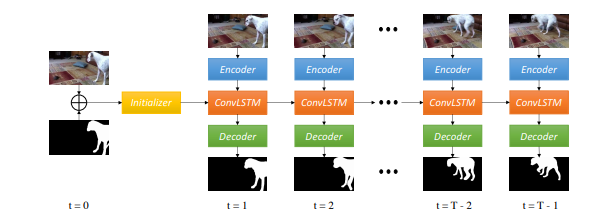
\includegraphics[scale=.6]{structure}
\caption{The structural skeleton of the proposed algorithm.}
\label{fig:structure}
\end{figure}

The input is passed through an encoder first from the video format. The outputs are put on the decoder to generate the annotations. The initial states of the inputs are generated by a feed forward NN which helps us encode the first frame x\textsubscript{0} and the segmentation mask y\textsubscript{0}. 
x\textsubscript{0} and y\textsubscript{0} are the forwarded into the \emph{Initializer}. It gives us the output for the t\textsubscript{0} memory state c\textsubscript{0} and hidden state h\textsubscript{0}. The outputs are fed into the ConvLSTM to learn the next sequence learning.
Time step = t, frame = x\textsubscript{t} is the outcome of the Encoder is \~{x\textsubscript{t}} which is a feature map. The ConvLSTM mentioned before takes this \~{x\textsubscript{t}} as input to capture the new characteristics from the video. We keep updating the internal states h\textsubscript{t} and c\textsubscript{t} based on the  \~{x\textsubscript{t}} since the model is compatible with back propagation. We pass the h\textsubscript{t} through the decoder to get the segmentation result \^{y\textsubscript{t}}. We use the binary cross entropy to calculate the loss between y\textsubscript{t} and \^{y\textsubscript{t}}. 
\newline
\newline
Functions:
\newline
\begin{equation} \label{eu_eqn}
c\textsubscript{0}, h\textsubscript{0} = \emph{Initializer}(x\textsubscript{0}, y\textsubscript{0})
\end{equation}
\begin{equation} \label{eu_eqn}
\~{x\textsubscript{t}} = \emph{Encoder}(x\textsubscript{t})
\end{equation}
\begin{equation} \label{eu_eqn}
c\textsubscript{t}, h\textsubscript{t} = \emph{ConvLSTM}(\~{x\textsubscript{t}}, c\textsubscript{t-1},h\textsubscript{t-1})
\end{equation}
\begin{equation} \label{eu_eqn}
\^{y\textsubscript{t}} = \emph{Decoder}(h\textsubscript{t})
\end{equation}
\begin{equation} \label{eu_eqn}
{\mathcal{L}} = -({y\textsubscript{t}log(\^{y\textsubscript{t}})) + ((1 - y\textsubscript{t})log(1 - \^{y\textsubscript{t}}}))
\end{equation}

Initializer and Encoder use VGG-16 structure with the conv layers that are fully connected. Then these layers are converted into 1 x 1 layer for the purpose of making the model fully convolutional. Initializer has two more ReLU layers that produce c\textsubscript{0} and h\textsubscript{0}. These layers have 512 filters. Sigmoid activation function is implemented for the stae outputs.  Decoder has 5 layers 5 x 5 kernel size, 512, 256, 128, 64 and 64. ConvLSTM layers use 512 3 x 3 filters. All these filters are initialized by Xavier. 

\vspace*{.5cm}
\section{Experiments}
\subsection{Training}
We train the model on a train-subset from YouTube VOS dataset because of the resource and time restrictions. So the score we would get from training the model on full dataset is understanbly higher than the one we got. 10 categories are elected for unseen category during testing process. The accuracy matrices contains $\mathcal{F}$ the contour accuracy and $\mathcal{J}$ as region similarities.
\newline
Here is a screenshot of the train sub-set
\begin{figure}[h!]
\centering
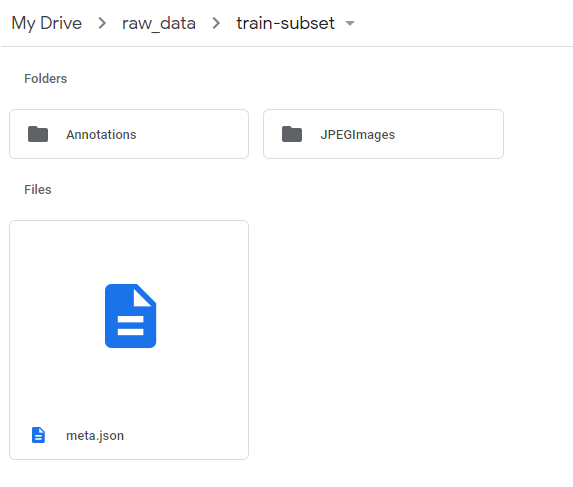
\includegraphics[scale=.6]{train sub.png}
\caption{Training sub-set.}
\label{fig:Training sub-set}
\end{figure}
As we have mentioned about the training subset, we trained our model on 50 epoch, in each epoch we calculated the Average Loss using the binary cross entropy as seen on figure 3. After the training process the model generates recons that are equal to the number of epoch, so we had 50 recons to visualize the models prediction of the given annotations from train-subset.from the recons we can see how the model gradually improves with time and more with training. 
\begin{figure}[h!]
\centering
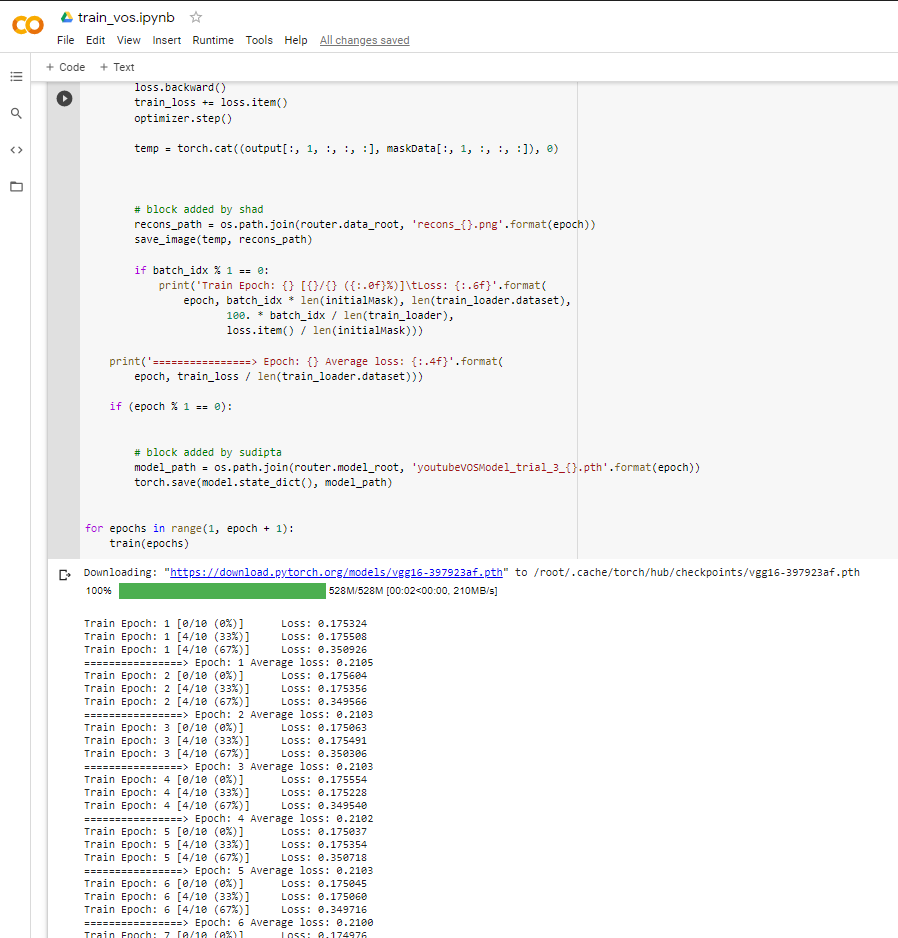
\includegraphics[scale=.3]{train_code.png}
\caption{Training process of the model and calculating the average loss.}
\label{fig:train_code}
\end{figure}
\newline
From these example we can get a better understanding.
\begin{figure}[h!]
\centering
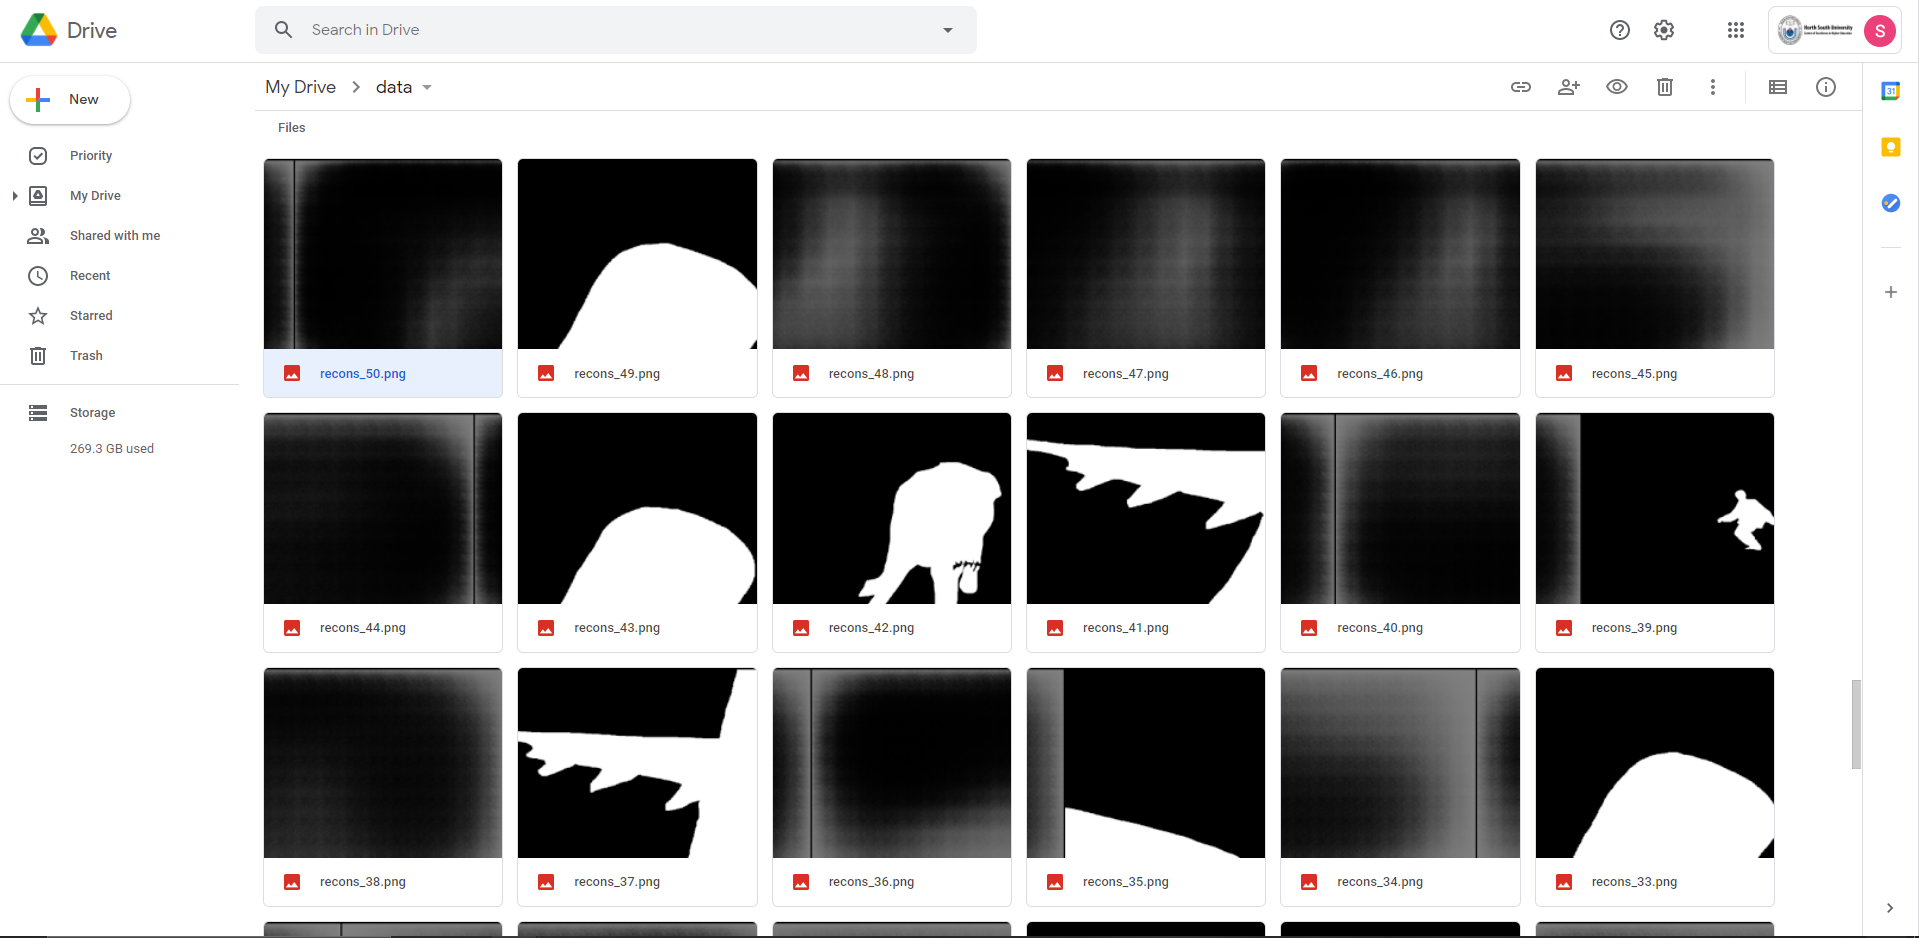
\includegraphics[scale=.18]{recons.png}
\caption{Producing recons.}
\label{fig:recons}
\end{figure}
\newline
Now if we see the very first recon on figure 5, we see the vast difference between the ground truth and the segmentation mask. This will improve over the course of training. For recon 25 on figure 6 we see some of that improvement. The model started to predict better than it did before. And on our final recon on figure 7 we see further improvement. 

\begin{figure}[h!]
\centering
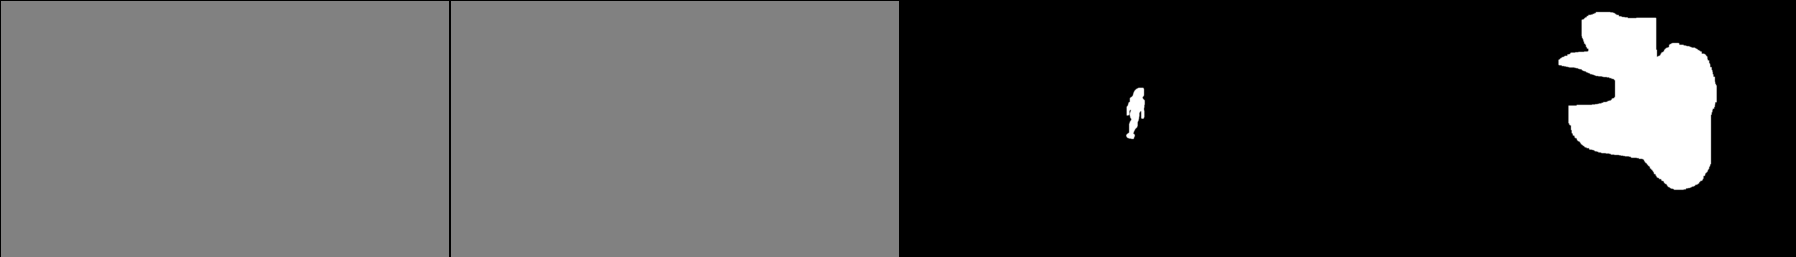
\includegraphics[scale=.18]{recon 1.png}
\caption{Recon 1.}
\label{fig:recons}
\end{figure}
\newline

\begin{figure}[h!]
\centering
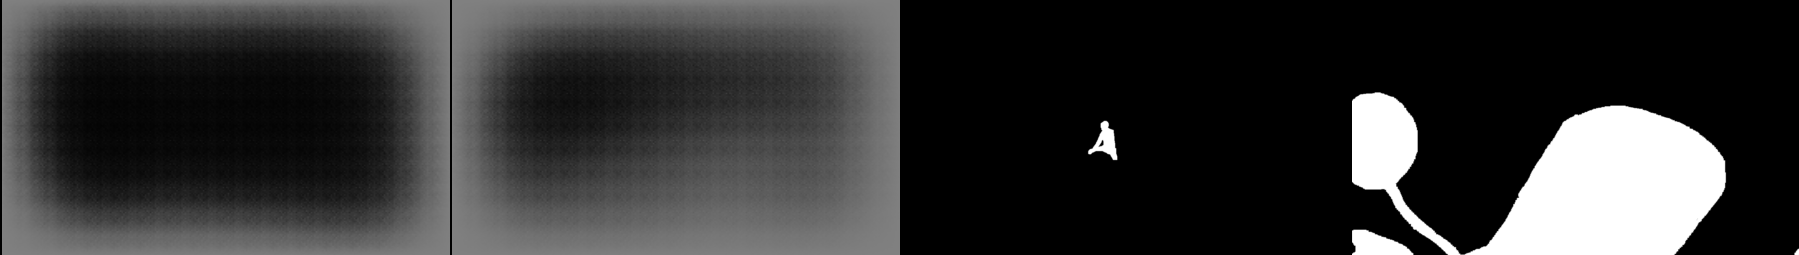
\includegraphics[scale=.18]{recon 25.png}
\caption{Recon 25.}
\label{fig:recons}
\end{figure}
\newline

\begin{figure}[h!]
\centering
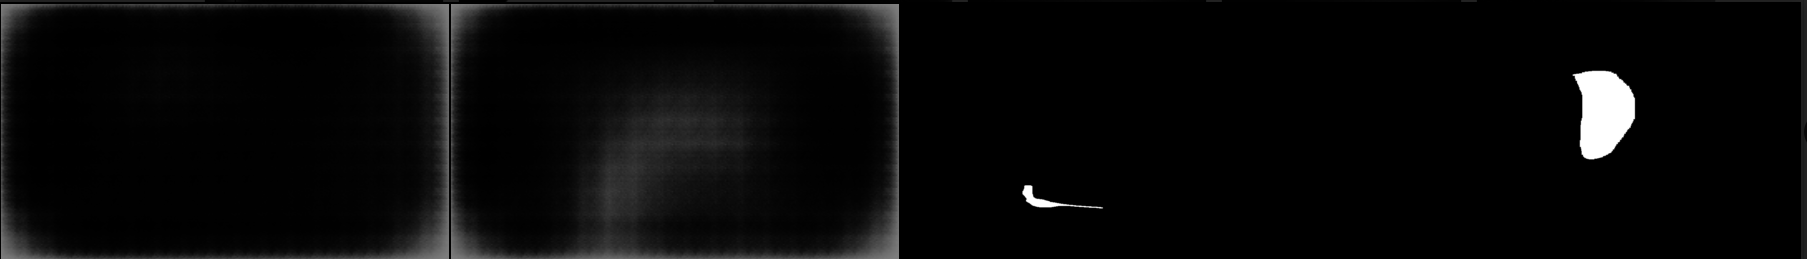
\includegraphics[scale=.18]{recon 50.png}
\caption{Recon 50.}
\label{fig:recons}
\end{figure}
\newline

\subsection{Validation}
From the YouTube VOS data set we also get a valid data set that is used to validate the model. We run the test on the entire data set. 
\begin{figure}[h!]
\centering
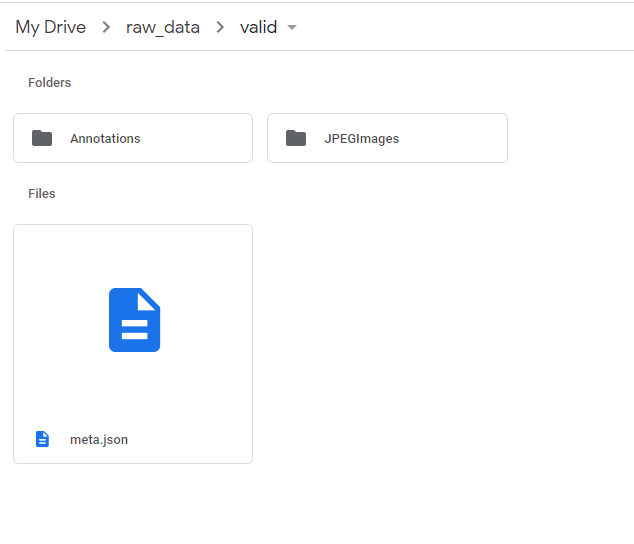
\includegraphics[scale=.5]{valid set.png}
\caption{Validation data}
\label{fig:recons}
\end{figure}
\newline
\begin{figure}[h!]
\centering
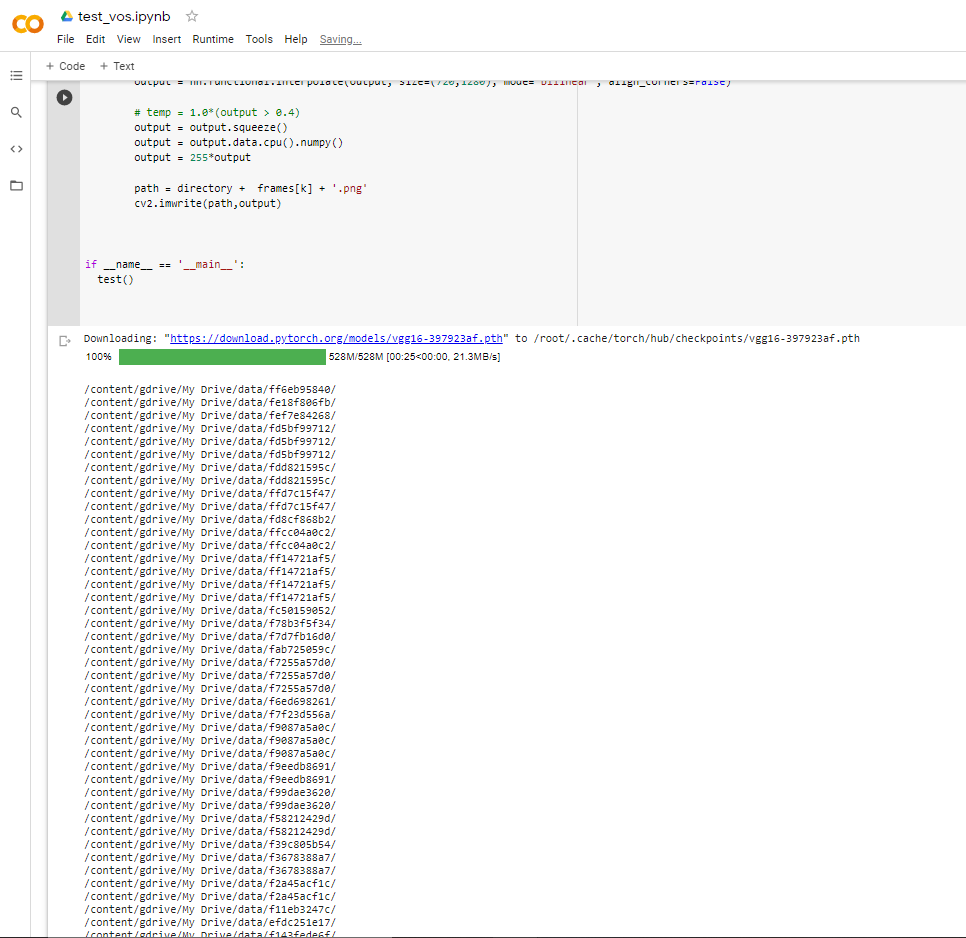
\includegraphics[scale=.5]{test_code.png}
\caption{Validation process}
\label{fig:recons}
\end{figure}
\newline
The validation set generate the annotations folders as shown in figure 10 from our model. We use those annotations to get the scores for accuracy matrices.

\begin{figure}[h!]
\centering
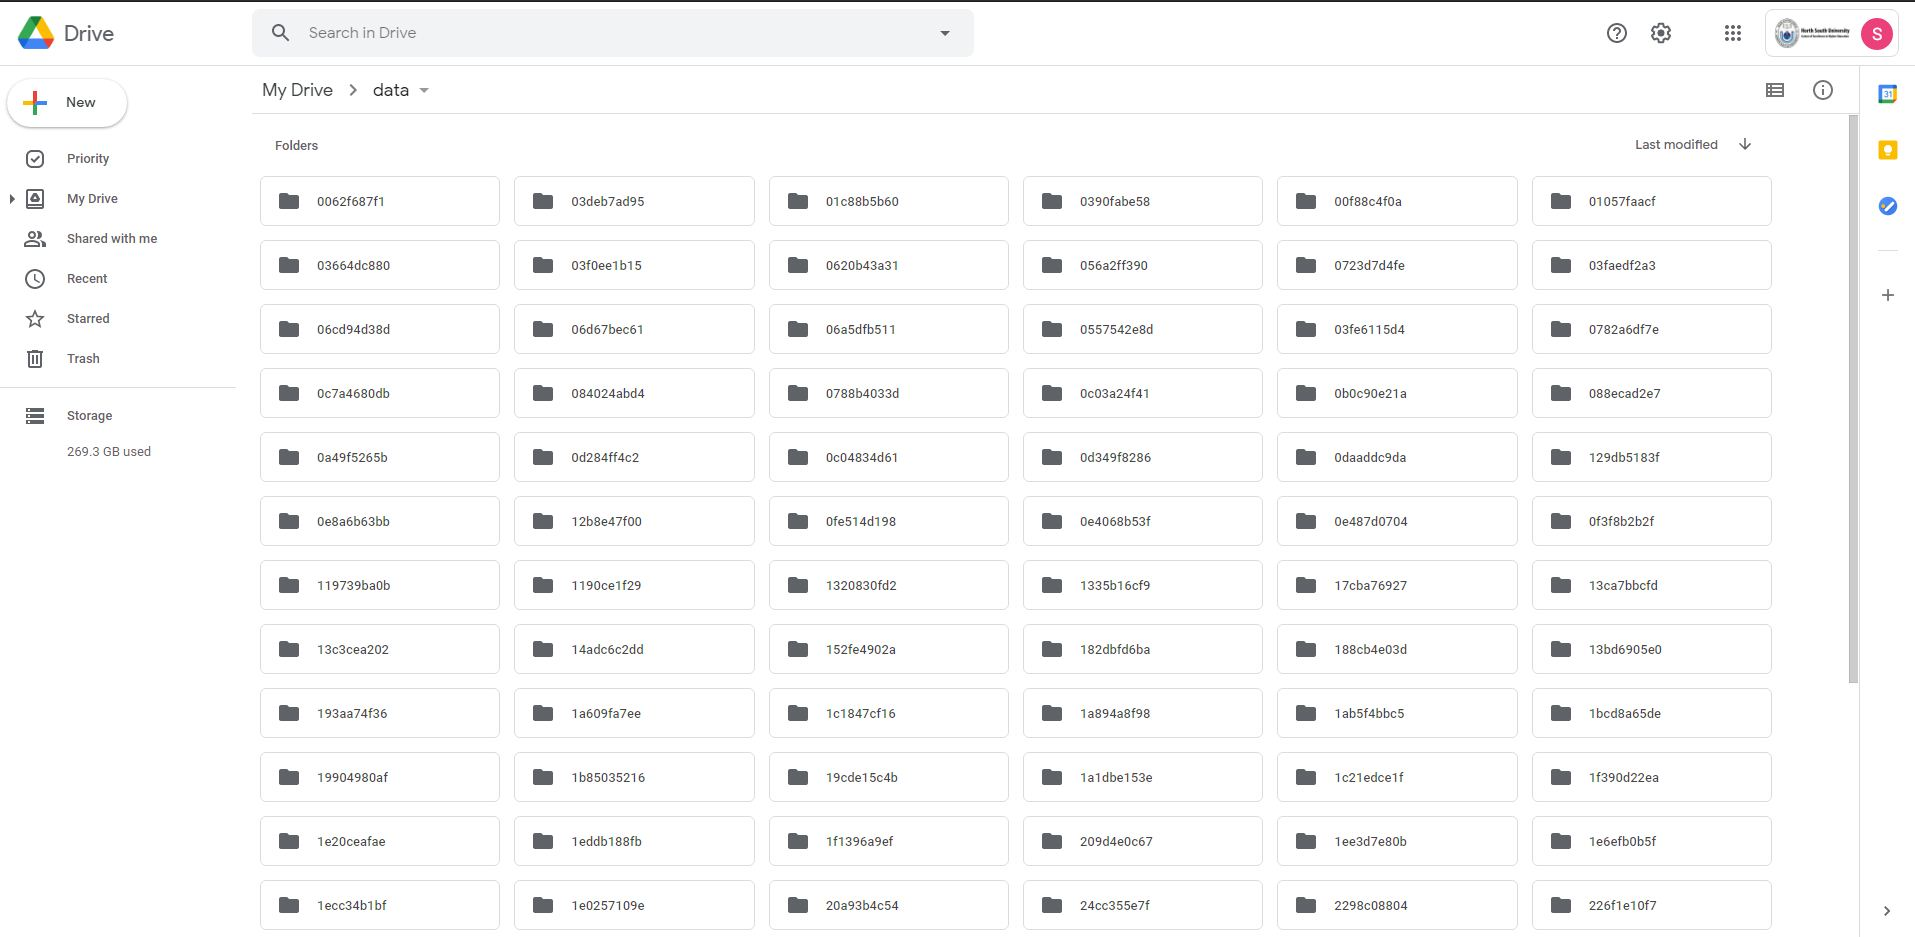
\includegraphics[scale=.16]{validation.JPG}
\caption{Annotation}
\label{fig:annotation}
\end{figure}

\vspace*{.5cm}
\section{Results}
We submitted our annotations in the CodaLab competition and got a score. We had difficulties with this because of the dimension error of training and testing phases but we managed to fix that and got a score from the website. 
\begin{figure}[h!]
\centering
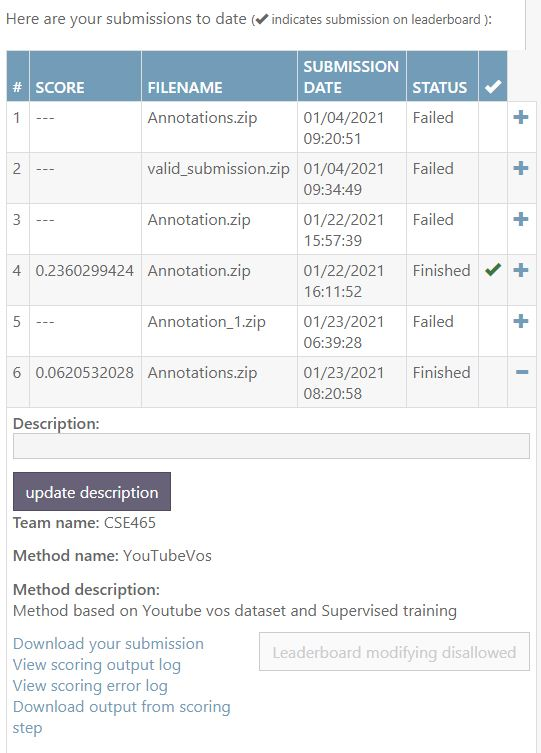
\includegraphics[scale=.5]{codalab.JPG}
\caption{Results}
\label{fig:results}
\end{figure}
Our accuracy matrices' given below\newline
Overall: 0.0620532027938\newline
$\mathcal{J}$ seen: 0.0474691634105\newline
$\mathcal{J}$ unseen: 0.0766372421771\newline
$\mathcal{F}$ seen: 0.0474691634105\newline
$\mathcal{F}$ unseen: 0.0766372421771\newline





\section{Conclusion}
Implementing the YouTube-VOS sequence-to-sequence Video Object Segmentation paper was definitely a challenge for us. With very limited processing power to train or test the model, we faced so many obstacles. Work in Google-Colab environment was a challenge while debugging the GitHub repo was more challenging. However, the approach we proposed was good enough to solve the tensor dimension issue with the test data. And that’s why we were able to implement the YouTube-VOS sequence-to-sequence Video Object Segmentation paper. There are still a lot of places to improve the implantations. We believe our work will help a bunch of people who faced the tensor dimension issues with that particular GitHub repository.


\bibliographystyle{plain}
\bibliography{references}

\vspace{12pt}


\end{document}
